\chapter{Migration Jira/Java Correction WorkBench}\label{chapitre:migration}

\section{Qu'est-ce que Jira et Java Correction WorkBench (JCWB)}
Jira\index{Jira} est un logiciel de tra\c{c}abilit\'{e} des probl\`{e}mes d\'{e}veloppé par Atlassian dont l'usage est gratuit pour les organisations \`{a} but non lucratif, de charit\'{e} ou les projets open-source. SAP désire migrer de système de traçabilité pour utiliser maintenant Java Correction WorkBench\index{Java Correction WorkBench} (JCWB ou CWB).\\

JCWB est un logiciel interne à SAP dont l'utilisation à été imposée par la hiérarchie, son domaine d'utilisation est la gestion des corrections. Historiquement, SAP utilise Jira pour gérer le projet, les problèmes (defects) et les corrections.\\
La stratégie de gestion des bugs changeant, SAP a pris la décision d'utiliser un seul et même outil de gestion des problèmes en interne comme en externe (à l'usage des clients) : BCP. Cet outil permet de renseigner un problème, quel qu'il soit, et s'il s'avère que ce problème est un bug logiciel il est transféré vers JCWB, qui suivra ce bug toute la durée de la correction.

%ASTEC est un logiciel interne à SAP dont la première version est sortie en 2007. ASTEC



\section{Pr\'{e}sentation du contexte}


\`{A} SAP, tous les codes des différents projets sont hébergés sur le gestionnaire de version Perforce\index{Perforce} (SCM : Source Code Management)
et ceux-ci sont compilés plusieurs fois par jour grâce à Jenkins\index{Jenkins} ou ASTEC (CIS : Continuous Integration Software).\\
Chaque projet est constitué de deux choses distinctes, d'une part, son code source et, d'autre part, les tests joués pour garantir\footnote{La valeur de la garantie dépend directement du test coverage} le bon fonctionnement du produit. Lorsqu'il y a un problème sur la build, que ce soit une erreur de compilation ou un test qui échoue, le statut de la build change pour être représentatif du problème. Dès lors que quelqu'un s'en aperçoit, il inscrit un defect\index{Defect} dans Jira\footnote{L'utilité de Jira est bien plus large que la simple déclaration d'un test échoué, il sert à décrire n'importe quel problème quelle que soit la version, la branche ou le produit} ou dans JCWB.\\


\subsection{Plugin de reporting}
Pour leur permettre d'avoir un rapport visuel sur l'état des builds, ils utilisent le plugin Radiator. Ce plugin permet l'affichage, sur un seul écran divisé, des groupes de jobs\footnote{Typiquement, un job correspond à un projet logiciel}. Un groupe de jobs est un carré coloré dont la couleur représente l'état des jobs qui le compose, voir la capture d'écran figure \ref{figure:radiatorActual} page \pageref{figure:radiatorActual}.\\
Les statuts pris en compte sont les statuts Jenkins\footnote{Error, Failure, Unstable, Aborted, Not built, Success} ainsi qu'un statut supplémentaire issue du plugin Claim. Ce plugin permet à un développeur de \textquote{claimer} une erreur, c'est-à-dire, ajouter au projet une information supplémentaire : le nom de l'utilisateur qui a \textquote{claimer} et le message que celui-ci a laisser aux visiteurs suivants.




\begin{figure}[!h]
  \centering
      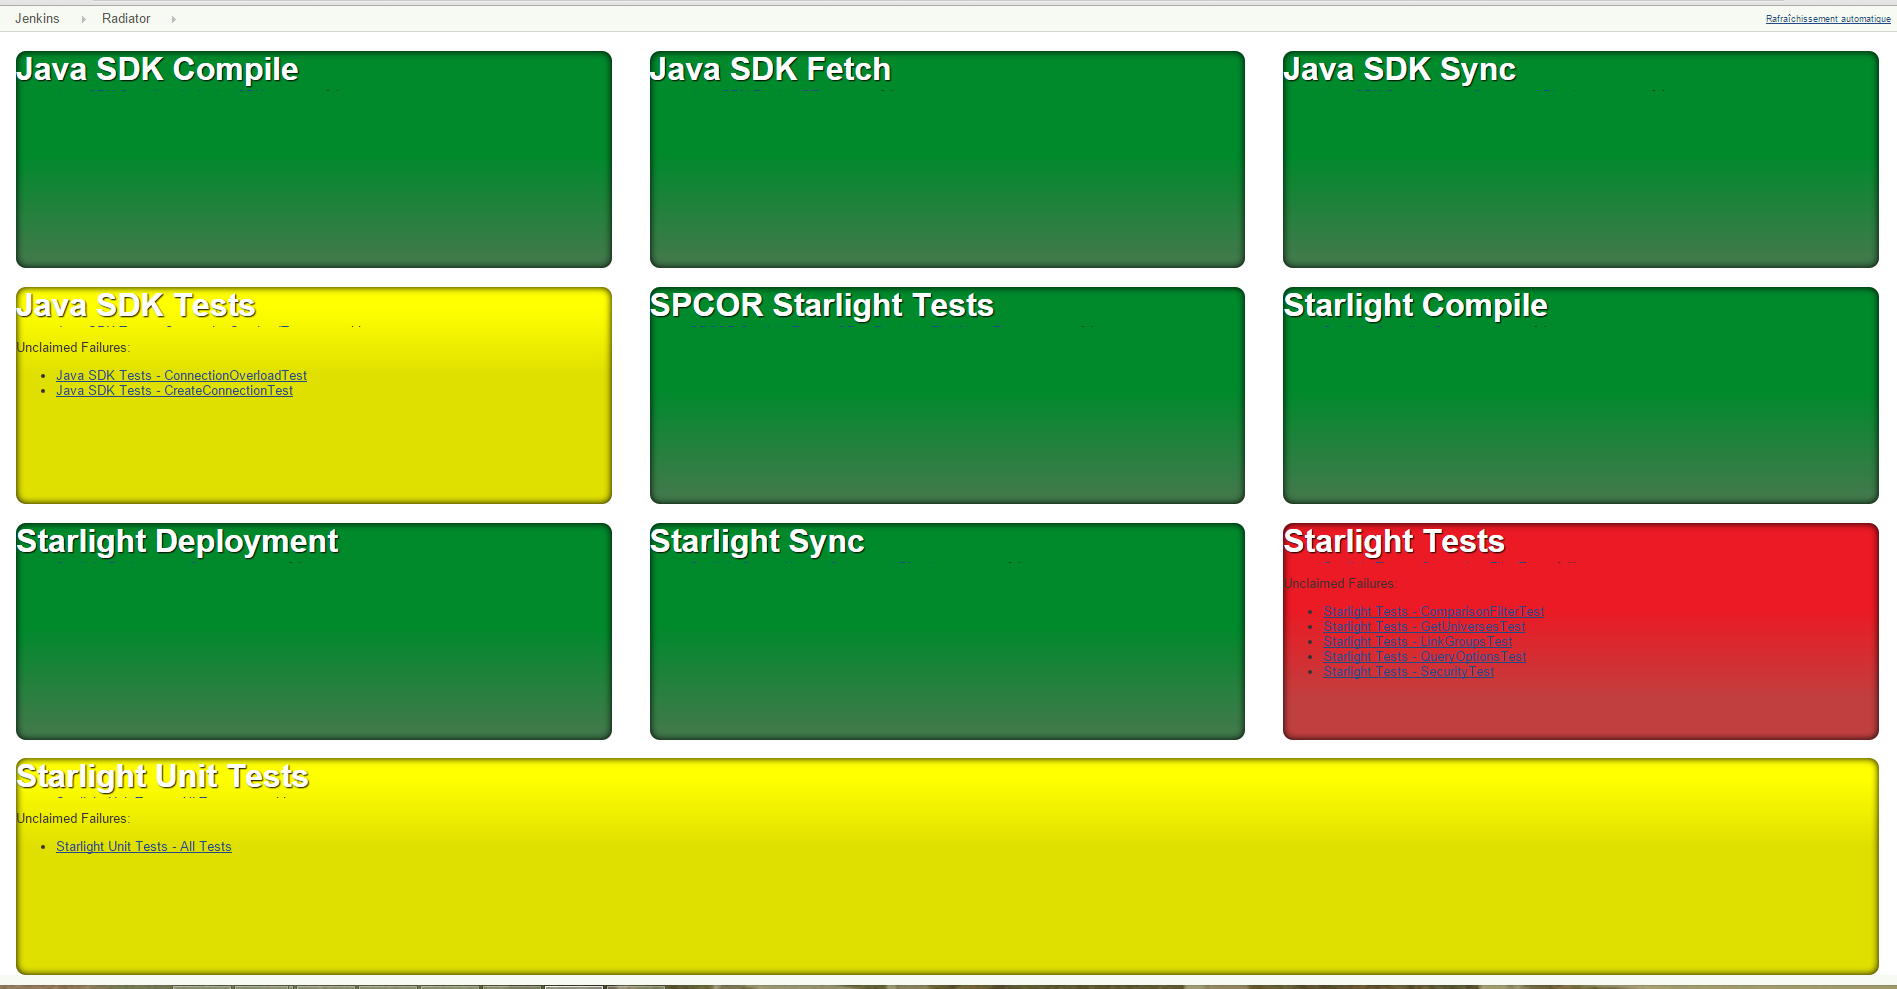
\includegraphics[width=\textwidth]{images/radiatorActual.png}
  \caption{Plugin Radiator utilisé actuellement}
	\label{figure:radiatorActual}
\end{figure}

En résumé Radiator :
\begin{itemize}
	\item permet de rassembler les jobs en un seul groupe de jobs
	\item où chacun des jobs a un statut\footnote{statut propre à Jenkins}
	\item que le groupe de projet arbore la couleur représentative du statut jugé le plus important
	\item permet de prendre en compte les informations supplémentaires du plugin claim
\end{itemize}
Par exemple, si nous avons deux groupes composés chacun de trois jobs, tous différents. Supposons que, sur les 6 jobs, l'un soit en échec les autres étant en succès. Nous aurons donc une vue colorée en verte (parce que tous les projets sont en succès) et la deuxième vue apparaissant en rouge (l'un des jobs ayant échoués) ou bien en orange si l'échec est investigué (échec claim par un développeur).\\
La figure \ref{figure:RadiatorInformationSources} page \pageref{figure:RadiatorInformationSources} illustre bien les sources d'informations du plugin. Il puise ses résultats depuis Jenkins et le plugin claim, les résultats de Jenkins puisant ses résultats en partie des résultats de tests JUnit.\\
L'inconvénient de ce procédé est que lorsque qu'un test a échoué, tout le groupe de test passe en rouge. Dans cette situation, il devient impossible de détecter les nouveaux tests qui échouent.




\begin{figure}[!h]
  \centering
      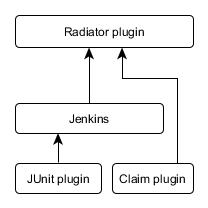
\includegraphics[scale=0.5]{images/RadiatorInformationSources.jpg}
  \caption{Contexte du'utilisation du plugin Radiator utilisé actuellement}
	\label{figure:RadiatorInformationSources}
\end{figure}




La solution simple et provisoire, mais permettant de contourner le problème et de ne plus polluer l'affichage avec du rouge, consiste à faire passer les jobs en échec avec defect\index{Defect} (ie. reconnus et enregistrés comme échecs dans Jira\index{Jira} ou CWB\index{Java Correction WorkBench}) en vert.\\
De cette manière, puisque seuls les nouveaux échecs apparaissent en rouge, toute régression est visible immédiatement.\\
Cette transformation est mise en \oe{}uvre grâce à une annotation, celle-ci est présentée figure \ref{figure:annotationJava} page \pageref{figure:annotationJava}.\\


\begin{figure}[h]
  \centering
      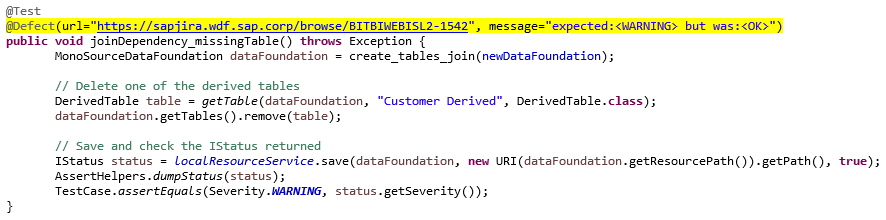
\includegraphics[width=\textwidth]{images/annotationJava.png}
  \caption{Annotation utilisée pour vérifier le statut du defect Jira}
	\label{figure:annotationJava}
\end{figure}

De cette manière le test est relié au defect et si :
\begin{enumerate}
	\item le test est échoué mais le statut est \textquote{Active} ou \textquote{Open}
	\item le message d'erreur match\footnote{} avec celui attendu
\end{enumerate}
\textbf{Alors}, le test sera considéré en succès par Jenkins. Ensuite, quand un développeur livrera le fix, le defect passera à \textquote{Validate}, ce qui court-circuitera l'annotation\footnote{même comportement pour le statut \textquote{Closed} ou n'importe quel autre qui n'est pas \textquote{Active} ni \textquote{Open}}. Et en fonction de l'efficience du fix, le test redevient vert ou reste à rouge.\\
\textbf{De cette manière}, seuls les tests non investigués sont rouges, ce qui permet de réagir beaucoup plus rapidement et de réduire le temps d'investigation.\\

Pour résumer, la relation qu'entretien BCP et JCWB est illustrée figure \ref{figure:bugManagementProcess}.

\begin{figure}[h]
  \centering
      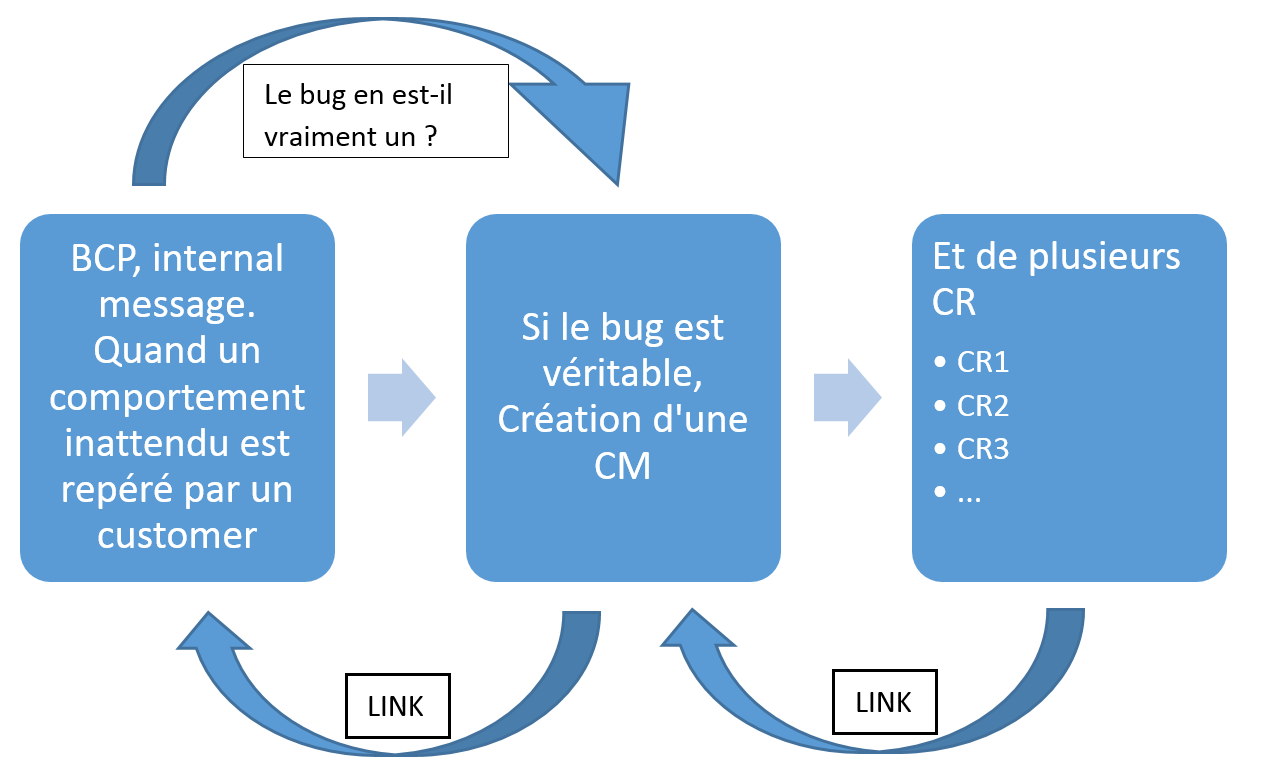
\includegraphics[width=\textwidth]{images/bugManagementProcess.png}
  \caption{Process de gestion de bug utilisé}
	\label{figure:bugManagementProcess}
\end{figure}




\textbf{Problématique}\hfill \\ \indent

Actuellement, seuls les defects rentrés sur Jira sont pris en compte, la mécanique en place ne permet pas de récupérer ces mêmes informations de JCWB\index{Java Correction WorkBench}. \\
Puisque de plus en plus de defects seront enregistrés sur JCWB, et dans un soucis d'homogénéisation du process actuel, il faut mettre à jour le process actuel et permettre aux statuts d'être ajustés quelque soit l'origine du defect (Jira ou CWB).\\
La problèmatique supplémentaire relève de l'architecture différente différente de Jira et de BCP\footnote{Contient le message initial à l'origine du defect} + JCWB\footnote{Contient la \textquote{Correction Measure} (CM) et les \textquote{Correction Requests}} (CR), ce qui nous oblige à aller receuillir des informations à deux endroits différents. Le premier objectif étant de récupérer l'identifiant de la \textquote{Correction Request} à laquel le defect est associé et l'identifiant de la \textquote{Correction Measure} à laquel la CR est associée.\\






\section{Travail effectué}


La première partie du travail s'est cantonée d'abord à des échanges de mails parallèlement à des recherches.\\
Les différentes choses essentielles à mon projets sont les suivantes :

\begin{itemize}
	\item il existe un web service permettant de récupérer les informations d'une CR : CWB HTTP API
	\begin{itemize}
		\item l'utilisation de ce web service se fait via une authentification normalisée par SAP : PROD-PASS-ACCESS
	\end{itemize}
	\item le fichier à implémenter pour compléter le comportement actuel est JiraIssueWatcher.java	
\end{itemize}




\subsection{Fonctionnement et utilisation de prod-pass-access}



\subsection{Son utilisation depuis Java}



\section{Résultats obtenus}
Maintenant cette mission achévée, nous pouvons récupérer les informations relatives au statut d'un defect, quelque soit son emplacement (Jira ou CWB), depuis test-defects.xml.



-> connaissances Java
J'ai approfondi mes connaissances sur les annotations et la manière de les implémenter.
J'ai implémenté ma première classe abstraite 

